\documentclass{article}
\usepackage[T1]{fontenc}
\usepackage{graphicx}
\usepackage{color}
\usepackage{amsmath}
\usepackage{caption}
\usepackage{wrapfig}

\title{\Large{CSE300\textunderscore Assignment1 \\ 
    Introduction to \LaTeX} \\ 
    \Huge{Elasticity of Materials} }

\large{ 
\author{Abdullah Al Ishtiaq \\
    Student ID: 1505080 }
}

\date{}

\begin{document}

\maketitle

\vspace{4cm}

\begin{figure}[h!]
\centering
    
\includegraphics[width = 0.25\textwidth]{Figures/logoBUET.png}
\end{figure}
\begin{center}

\vspace{.5cm}

\Large{Department of Computer Science and Engineering \\
    Bangladesh University of Engineering and Technology \\
    (BUET) \\
    Dhaka 1000 \\
    \date{\today} }

\end{center}


\newpage

\tableofcontents
\newpage

\section{Introduction}

    Every physical body is made up of either atoms or molecules. These particles are attracted to one another through inter-molecular forces. When force is applied on a body to deform its shape, the inter-molecular forces try to retain its original shape. Thus the term \textit{Elasticity} is introduced.\\

    In physics, \textit{elasticity} is the ability of a body to resist a distorting influence and to return to its original size and shape when that influence or force is removed. Solid objects will deform when adequate forces are applied on them. If the material is elastic, the object will return to its initial shape and size when these forces are removed.

    \subsection{Some Important Definitions}

        \begin{description}

            \item[\textcolor{blue}{Elastic Limit:}]    
                The maximum extent to which a solid may be stretched without permanent alteration of size or shape is called its Elastic Limit.
            
            \item[\textcolor{blue}{Perfect Elastic Body:}]    
                Perfect elastic body is an ideal concept. A physical body which always returns to its original shape after removing the applied force which cause its deformation is called a perfect elastic body.

            \item[\textcolor{blue}{Perfect Plastic Body:}]    
                Perfect plastic body is also an ideal concept. A physical body which always retains deformed shape after removing the applied force which cause its deformation is called a perfect plastic body.
            
            \item[\textcolor{blue}{Strain:}]  
                Strain is the ratio of change in dimension to the original dimension of the specimen , after the application of external force. \\
                For example, if original dimension of a body is A, and B is the dimension after applying the external force,
                \begin{equation}
                    strain = \frac{A \sim B}{A}
                    \label{subsec:strain}
                \end{equation}
                
            \item[\textcolor{blue}{Stress:}]  
                The stress is the force applied to per unit area of the material. It is defined as,
                \begin{equation}
                    stress = \frac{Force}{Area} = \frac{F}{A}
                    \label{subsec:stress}
                \end{equation}
            
            \item[\textcolor{blue}{Breaking Stress:}] 
                The maximum stress a material can stand before it breaks is called the breaking stress or ultimate tensile stress.
            
            \end{description}

    \subsection{Elastic Properties of a Matter and Inter-molecular Forces}
        Inter-molecular forces are produced mainly because of two kinds of energy:
        
        \begin{enumerate}
            \item Potential energy due to interaction of surrounding molecules.
            \item Thermal energy which is actually kinetic energy of the molecules.
        \end{enumerate}
        
        \begin{wrapfigure}{R}{0.3\textwidth}
            \centering
            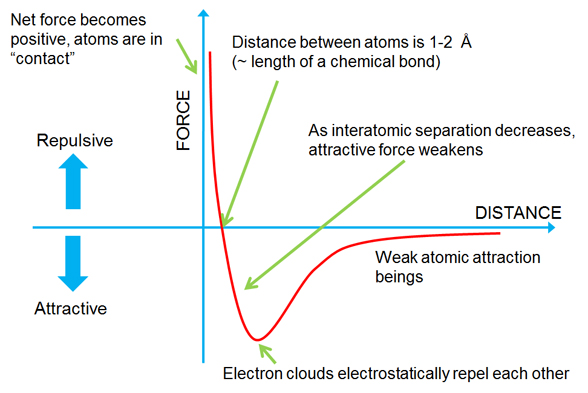
\includegraphics[width=0.5\textwidth]{Figures/ForceVsDistance.jpg}
            \caption{inter-molecular Force VS Inter-molecular Distance}
        \end{wrapfigure}    
            
        We can easily understand elasticity if we consider molecular shape of a matter. Normally molecules of a crystal stay in the position of the lowest potential energy. It is the equilibrium state. When inter-molecular distance is increased from the equilibrium distance, attractive force is introduced, and when distance is decreased from the equilibrium distance, repulsive force is introduced. Thus when the applied force which changed the distance is removed, molecules start to retain their original position, and so elasticity is produced.
        
\section{Different Types of Strain and Stress}
    According to definition from section \ref{subsec:strain} we can find different types of Strain and Stress.
    
    \subsection{Longitudinal or Tensile}
        \begin{itemize}
            \begin{figure}[h]
                \centering
                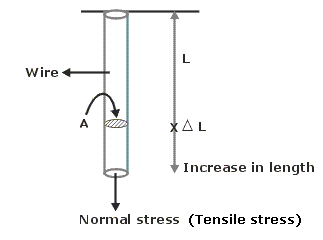
\includegraphics[width=.4\textwidth]{Figures/TensileStrain.png}
                \caption{Tensile Stress}
            \end{figure}
            \item \textcolor{blue}{\textbf{Longitudinal Strain:}}  \\
                If external force is applied on a physical body such that its length is changed, then the change along its length per unit length is called \textit{longitudinal strain}.
                    \begin{equation}
                        Longitudinal~Strain  = \frac{l}{L}
                    \end{equation}
            \item \textcolor{blue}{\textbf{Longitudinal Stress:}}  \\
                Force applied to per unit area to cause longitudinal strain is called \textit{longitudinal stress}.
        \end{itemize}

        
    \subsection{Volume or Bulk}
        \begin{itemize}
            \begin{figure}[h]
                \centering
                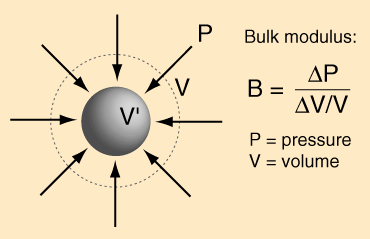
\includegraphics[width=.4\textwidth]{Figures/BulkStrain.png}
                \caption{Tensile Stress}
            \end{figure}
            \item \textcolor{blue}{\textbf{Bulk Strain:}}  \\
                If external force is applied on a physical body such that its Volume is changed, then the change in its volume per unit volume is called \textit{bulk strain}.
                    \begin{equation}
                        Bulk~Strain  = \frac{v}{V}
                    \end{equation}
            \item \textcolor{blue}{\textbf{Bulk Stress:}}  \\
                Force applied to per unit area to cause bulk strain is called \textit{bulk stress}.
        \end{itemize}
        
    \subsection{Shearing}
        \begin{itemize}
            \begin{figure}[h]
                \centering
                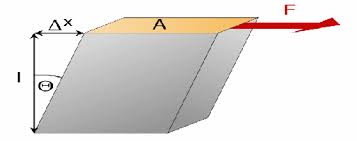
\includegraphics[width=.4\textwidth]{Figures/ShearStrain.jpg}
                \caption{Shearing Stress}
            \end{figure}
            \item \textcolor{blue}{\textbf{Shearing Strain:}}  \\
                \textit{Shear strain} is defined as the tangent of the angle of deformity, and is equal to the length of deformation at its maximum divided by the perpendicular length in the plane of force application.
                    \begin{equation}
                        Shearing~Strain  = \tan{\theta}
                    \end{equation}
            \item \textcolor{blue}{\textbf{Shearing Stress:}}  \\
                Force applied to per unit area to cause shearing strain is called \textit{shearing stress}.
        \end{itemize}
       
    

\section{Elastic Moduli}
    \subsection{Hooke's Law}
        English physicist Robert Hooke(1635-1703) has experimentally shown that stress of a body is proportional to strain within elastic limit. 
        \begin{equation}
            stress \propto strain
        \end{equation}
        or, 
        \begin{equation}
            \frac{stress}{strain} = constant
            \label{eqn:hook}
        \end{equation}
    
    \subsection{Different Moduli}
        From  equation \ref{eqn:hook} we know that the ratio of stress and strain is a constant number. This constant is elastic modulus of a body.
        
        Different types of stress and strain yields to different types of elastic moduli. They are as follows:
        
        \begin{description}
        
            \item[\textcolor{blue}{Young's Modulus:}]
                The ratio of longitudinal stress and the longitudinal strain within the elastic limit is a constant. This constant is called \textit{Young's Modulus}.
                    \begin{equation}
                        Y = \frac{longitudinal~stress}{longitudinal~strain} = \frac{FL}{Al} = \frac{MgL}{\pi r^2}
                        \label{eqn:modulusY}
                    \end{equation}
                
            \item[\textcolor{blue}{Bulk Modulus:}]
                The ratio of bulk stress and the bulk strain within the elastic limit is a constant. This constant is called \textit{bulk Modulus}.
                    \begin{equation}
                        B = \frac{bulk~stress}{bulk~strain} = \frac{FV}{Av} = \rho \frac{V}{v}
                    \end{equation}
                
            \item[\textcolor{blue}{Modulus of Rigidity:}]
                The ratio of shearing stress and the shearing strain within the elastic limit is a constant. This constant is called \textit{Modulus of Rigidity}.
                    \begin{equation}
                        \eta = \frac{shearing~stress}{shearing~strain} = \frac{F}{A\theta}
                    \end{equation}
                    
        \end{description}
        
        
\section{Work Done or Potential Energy stored for Stretching a Wire}
    \subsection{Total Work or Total Potential Energy}
        According to \textbf{work-energy theorem} work done in stretching a wire is stored as potential energy within the wire. \\
        Let, $L$ be the length and $A$ be the area of cross section of a wire. When $F$ force is applied, its length is increased by $dl$. So, work done, $dW = F dl$ 
        By integrating this equation from $l=0$ to $l=l$,
        \begin{equation}
            W = \int_{0}^{l} F~dl
            \label{eqn:intW}
        \end{equation}
        
        From equation \ref{eqn:modulusY},
        \begin{equation}
            F = \frac{YAl}{L}
        \end{equation}
        
        So, from equation \ref{eqn:intW},
        \begin{equation}
            W = \int_{0}^{l} \frac{YAl}{L}~dl
        \end{equation}
        
        By integration we can finally find,
        \begin{equation}
            W = \frac{1}{2}\frac{YAl^2}{L}
        \end{equation}
    
    \subsection{Potential Energy in Unit Volume}
        Total volume of the wire, $V = AL$. So, 
        \begin{equation}
            U = \frac{W}{V} = \frac{1}{2}\frac{YAl^2}{L} / AL = \frac{1}{2}\frac{Yl^2}{L^2}
        \end{equation}
        or, 
        \begin{equation}
                U = \frac{1}{2} Stress * Strain
        \end{equation}
        

\end{document}
